\part{Introduction}
In the school subject Model Based Design we designed our own solver for ODEs with the tools from MATLAB.
The tasks were usually not explained. Mostly only the questions were answered.

\part{Warming up}
	\section{Download}
	The following codesnippets where downloaded from Virtual Campus. The complet code with all adjustments is in the Appendix as Listing \ref{lst:ode1}.
	%
\begin{lstlisting}[caption={An abridged version of the Matlab code}, language=matlab, backgroundcolor = \color{lgray},label={lst:one}]
	%Startvalues
	y0 = 1;       % Initial condition of y
	t0 = 0;       % Initial time  
	tfinal = 10;  % Final time
	
	h = 1;        % Step size
	t = t0;                 % Actual time 
	i = 1;                  % Index counter 
	yk1(i,:) = [t0 y0 h];   % Matrix of result (first row)
	
	while 1                 % Infinite main loop
	
		% Forward Euler method (1st order)
		y1 = y0 + h*f(t,y0);
		
		% Updating values for next iteration
		y0 = y1;            
		i = i + 1;
		t = t + h;
		
		% Storing actual results
		yk1(i,:) = [t y1 h];
		
		% Ending condition
		if t > tfinal
			break;
		end    
	end			
\end{lstlisting}
		
		
		%
\begin{lstlisting}[caption={The funcion in the MATLAB code from Listing \ref{lst:one} row 14}, language=matlab, backgroundcolor = \color{lgray}]
	function [dydt] = f(t,y);		
		Tau=2;         
		dydt = -y/Tau;		
\end{lstlisting}
	The following differential equation from Equation \ref{eq:one} and \ref{eq:2} was solved with the FE method.
	
	\section{Run the downloaded Script}
		\begin{eqnarray}
			y_{k+1} &=& y_k + h * f(t, y) \label{eq:one }\\
			\frac{dy}{dt} &=& -\frac{y}{\tau} \label{eq:2}
		\end{eqnarray}

		
	\section{Understand the code}
		\subsection{Mainparameters}
	
			The main parameters are:  
			\begin{description}
				\item[\boldmath{$\tau$}] 	Defines the slope
				\item[y0] 		Is the startvalue
				\item[h] 		Is the stepsize
			\end{description}
		
		\subsection{Function}
			 The next point will be calculated with the actual point, the stepsize and the slope. This step by step in a loop until the defined end.
			


\newpage
\part{Analysis on solver precision}
	\section{Use }
		\subsection{Add the correct equation}
		In order to be able to compare the FE method, the antiderivative was added as a comparison value.
		
		
\begin{lstlisting}[caption={The antiderivative}, language=matlab, backgroundcolor = \color{lgray}, firstnumber=23]
	%4a
	y_t = y_start*exp(-t/Tau);
	yk2(i,:) = [t y_t h]; 
\end{lstlisting}				
		
		
		\subsection{Plot}
		In Figure \ref{fig:pl1}, the deviation of the FE method in comparison to the antiderivative is clearly visible. The red line is the FE method. The blue x's are the expected values.
		
			\begin{figure}[H]
				\centering
				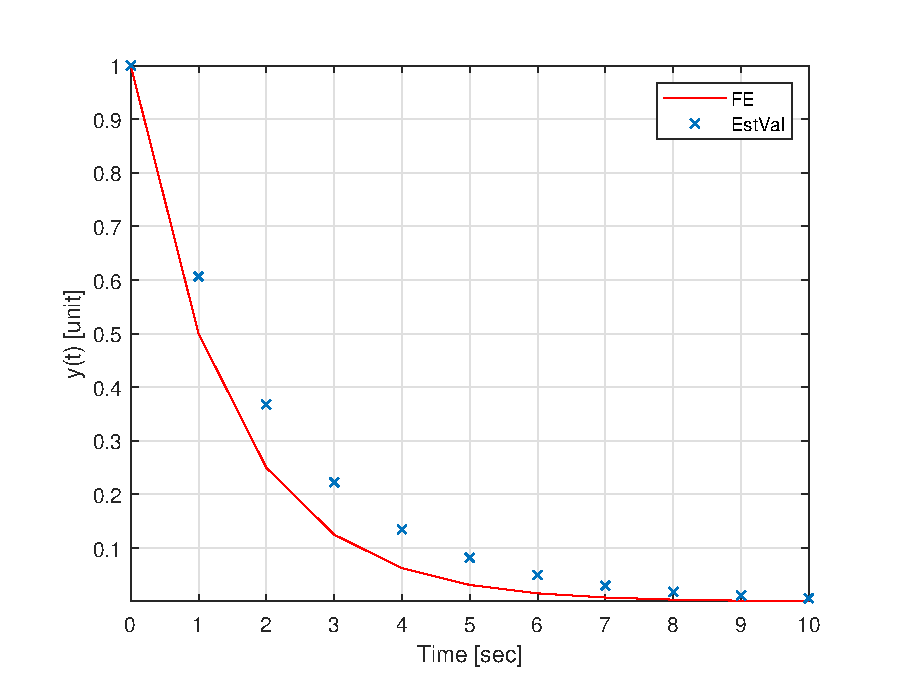
\includegraphics[width=0.7\textwidth]{graphics/fourb.eps}
				\caption{Comparison of FE method with the correct values from the derivative}
				\label{fig:pl1}
			\end{figure}
		
		
		\subsection{Difference between calculated and estimated value}
		The errors were calculated with the settings from List \ref{lst:param1}. In Table \ref{tb:arr1} are the values of the FE method, the expected values as well as the difference are to be read.

\begin{lstlisting}[caption={Parameters from the calculations}, language=matlab, backgroundcolor = \color{lgray}, label={lst:param1}]
	y0 = 1;       % Initial condition of y
	y02 = 1;
	t0 = 0;       % Initial time  
	tfinal = 10;  % Final time			
	h = 1;        % Step size
\end{lstlisting}			
			
			
%\begin{lstlisting}[caption={Create the following array}, language=matlab, backgroundcolor = \color{lgray}, firstnumber=23]
%	arr4 = [yk1(:,1), yk1(:,2), yk2(:,2), (yk2(:,2)-yk1(:,2))];
%\end{lstlisting}			

			\begin{center}
			$\begin{array}{cccc} 
				Time & Forward Euler & Correct Value & Difference \\
				 0 & 1.0 & 1.0 & 0\\ 1.0 & 0.5 & 0.607 & 0.107\\ 
				 2.0 & 0.25 & 0.368 & 0.118\\ 3.0 & 0.125 & 0.223 & 0.0981\\ 4.0 & 0.0625 & 0.135 & 0.0728\\ 
				 5.0 & 0.0312 & 0.0821 & 0.0508\\ 
				 6.0 & 0.0156 & 0.0498 & 0.0342\\ 
				 7.0 & 0.00781 & 0.0302 & 0.0224\\ 
				 8.0 & 0.00391 & 0.0183 & 0.0144\\ 
				 9.0 & 0.00195 & 0.0111 & 0.00916\\ 
				 10.0 & 9.77\,{10}^{-4} & 0.00674 & 0.00576\\ 
				 11.0 & 4.88\,{10}^{-4} & 0.00409 & 0.0036
			
			\end{array}$
			\captionof{table}{Values from Figure \ref{fig:pl1}}
			\label{tb:arr1}
			\end{center}

		\subsection{Error}
		The AATE (average absolute total error) was calculated with the code from Listing \ref{lst:err}. In addition, the RMSE (root mean square error)  was calculated. The RMSE has the advantage that it more weighted larger errors.
\begin{lstlisting}[caption={The funcion}, language=matlab, backgroundcolor = \color{lgray}, firstnumber=23, label={lst:err}]
	aate4 = sum(abs(arr4(:,4)))/(length(arr4)-1);
	rms4 = rms(arr4(1:end,4))	
\end{lstlisting}


	\newpage		
	\section{Values of h}\label{sec:val}
	In this section different h-values were tested and shown in Figure \ref{fig:pl2}. The values can be read as rms and aate in Table \ref{tb:err1}. In Figure \ref{fig:err} you can see the RMSE and AATE in dependence of h. 
		
			\begin{figure} [H]
				\begin{center}
					\begin{subfigure}{0.3\textwidth}
						\begin{center}
							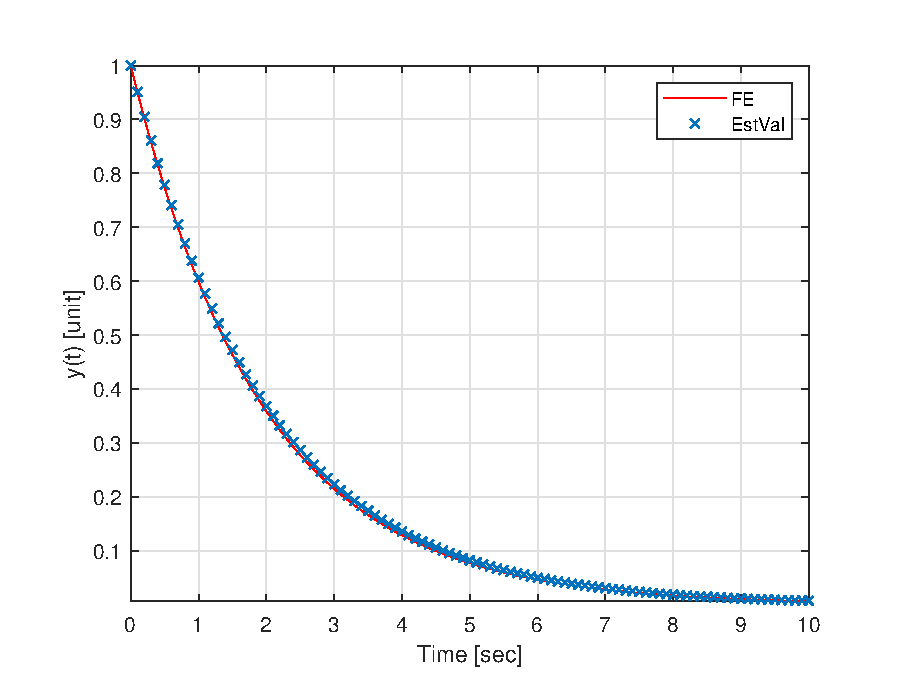
\includegraphics[width=1\textwidth]{graphics/fiveh0_1.eps}
						\end{center}
					\end{subfigure}
					\begin{subfigure}{0.3\textwidth}
						\begin{center}
							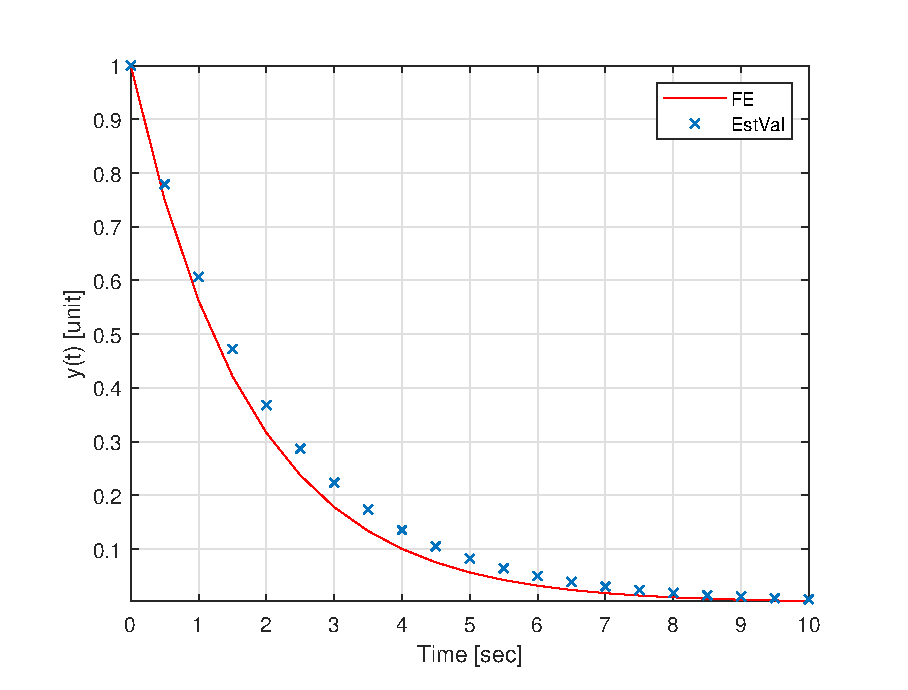
\includegraphics[width=1\textwidth]{graphics/fiveh0_5.eps}
						\end{center}
					\end{subfigure}
					\begin{subfigure}{0.3\textwidth}
						\begin{center}
							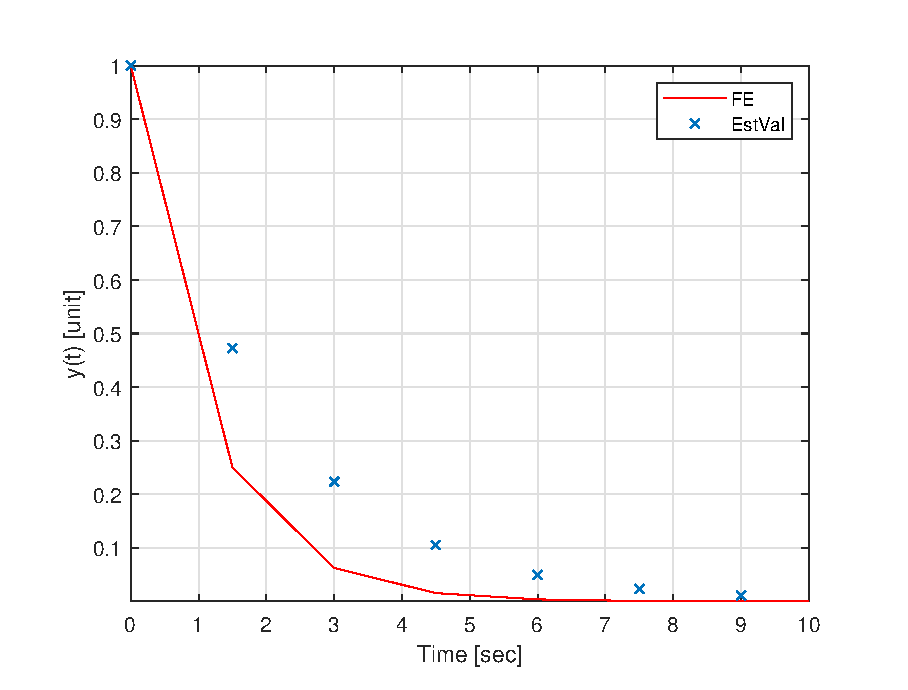
\includegraphics[width=1\textwidth]{graphics/fiveh1_5.eps}
						\end{center}
					\end{subfigure}
					\begin{subfigure}{0.3\textwidth}
						\begin{center}
							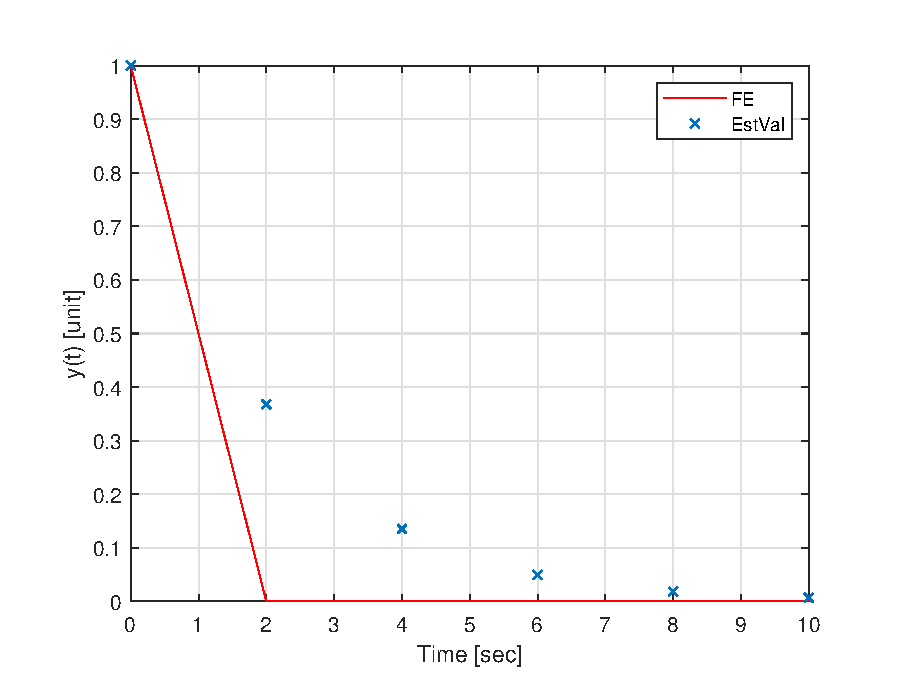
\includegraphics[width=1\textwidth]{graphics/fiveh2.eps}
						\end{center}
					\end{subfigure}
					\begin{subfigure}{0.3\textwidth}
						\begin{center}
							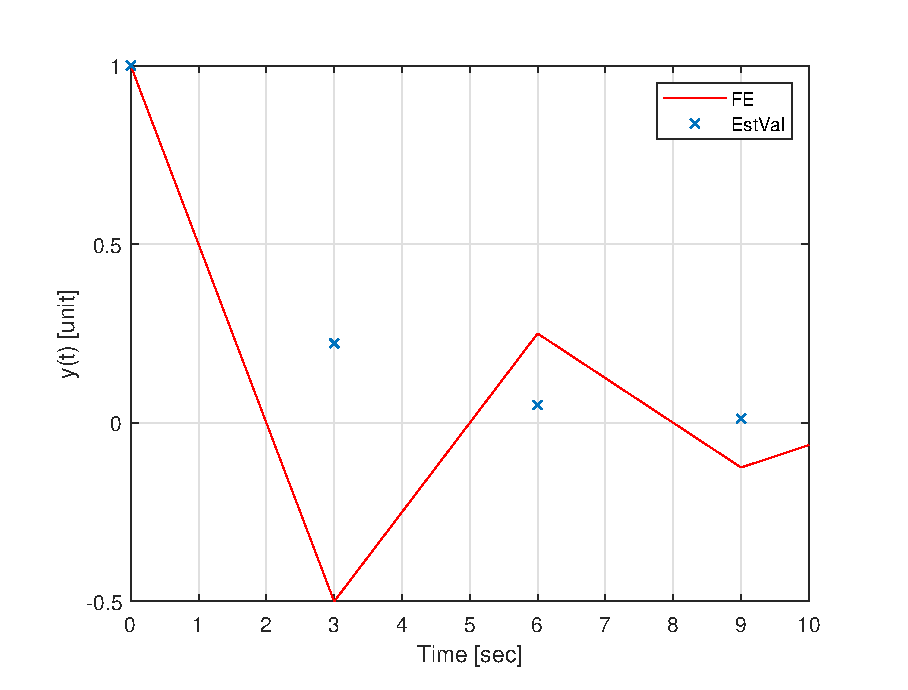
\includegraphics[width=1\textwidth]{graphics/fiveh3.eps}
						\end{center}
					\end{subfigure}
					\begin{subfigure}{0.3\textwidth}
						\begin{center}
							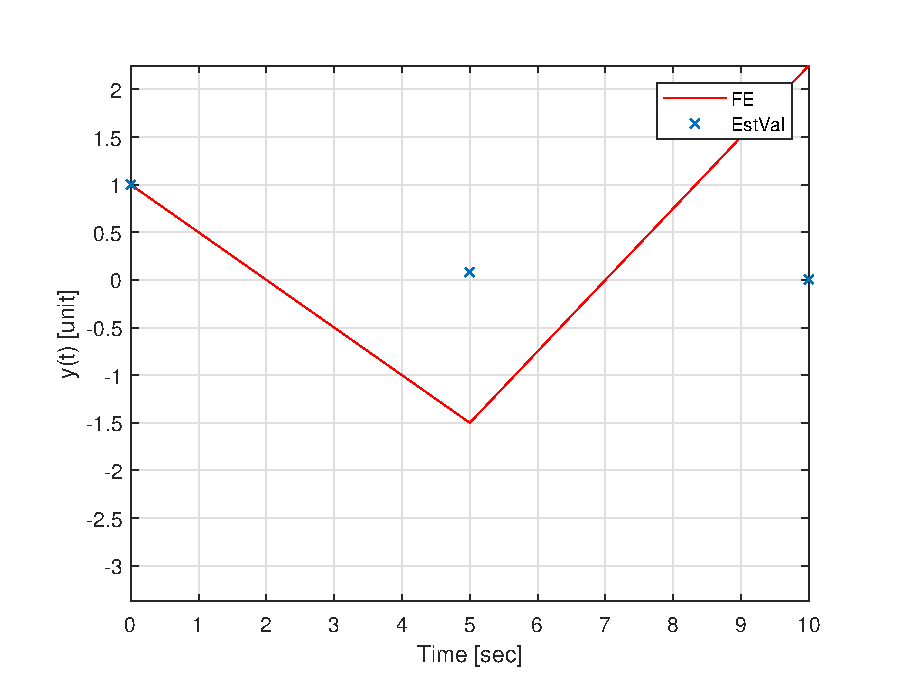
\includegraphics[width=1\textwidth]{graphics/fiveh5.eps}
						\end{center}
					\end{subfigure}
					\caption[Different h-values]{Different h-values. From top left: 0.1, 0.5, 1.5, 2, 3, 5}
					\label{fig:pl2}
				\end{center}
			\end{figure}
		
			\begin{table}[H]
				\begin{tabular}{c|cccccc}				
					& 0.1 & 0.5 & 1.5 & 2 & 3 & 5 \\ \hline
					\rowcolor{lgray}
					Average Absolute Total Error	& 0.0048 & 0.0243 & 0.0796 & 0.0968 & 0.2799 &  2.4003 \\ 
					Root Mean Square				& 0.0056 & 0.0289 & 0.1037 & 0.1495 & 0.3421 & 2.1754 \\ 
				\end{tabular}
				\caption{The errors from different h-values.}
				\label{tb:err1}
			\end{table}
		
			
			\begin{figure}[H]
				\centering
				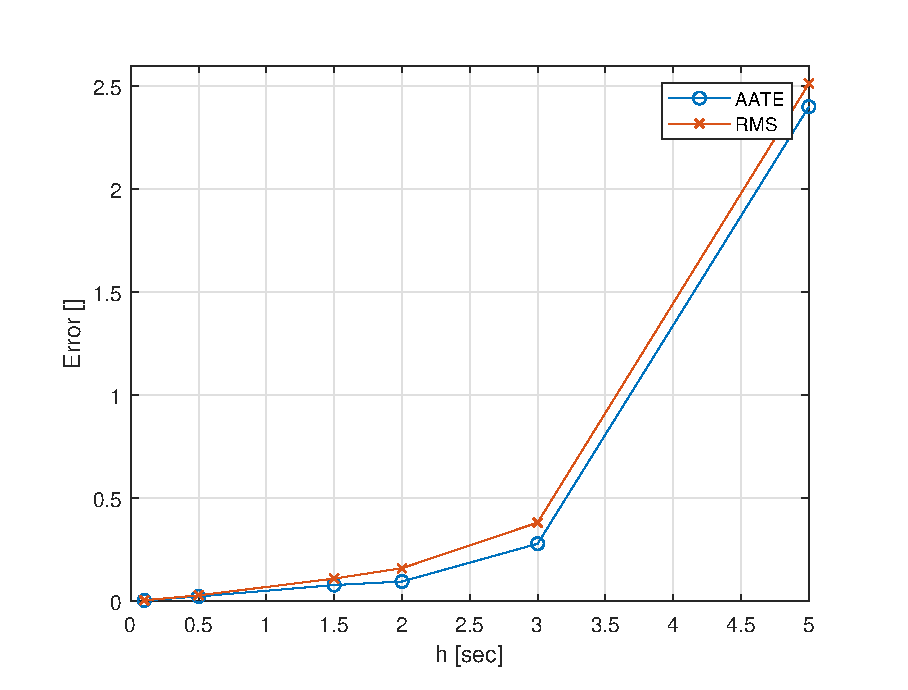
\includegraphics[width=0.7\textwidth]{graphics/error.eps}
				\caption{RMSE and AATE depending on h}
				\label{fig:err}
			\end{figure}
			
%			\begin{tikzpicture}
%				\begin{axis}[
%				title={Compare between AATE \& RMS},
%				xlabel={h},
%				ylabel={Error},
%				xmin=0, xmax=6,
%				ymin=0, ymax=3,
%				xtick={1, 2, 3, 4, 5},
%				ytick={1, 1.5, 2, 2.5},
%				legend pos=north west,
%				ymajorgrids=true,
%				grid style=dashed,
%				]
%				
%				\addplot[
%				color=blue,
%				mark=square,
%				]
%				coordinates {
%					(0,0)(0.1,0.0056)(0.5, 0.0289)(1.5, 0.1037)(2, 0.1495)(3, 0.2799)(5,  2.4003)
%				}			{(0,0)(0.1,0.0048)(0.5, 0.0243)(1.5, 0.0796)(2, 0.0968)(3, 0.3421)(5,  2.1754)};
%				\legend{AATE}{RMS}
%				
%				\end{axis}
%			\end{tikzpicture}
			
			

		
		\subsection{Influence of h}
		The smaller h, the more accurate the values of the FE method. This requires more computing power.
		
		\subsection{Good value for h}
		The smaller the h the smaller the error.
		
		\subsection{Oscilation and correlation between $\tau$ and h}
		The oscilastion starts when h > $\tau$. Because the step is taller than the slope and so the graph crosses the zeroline what is never excpacted with this equation and the graph starts to oscillate.

		
					

\part{Creating a general purpose solver}

	\section{Runge-Kutta}
		\subsection{Mid-Poind-Method Code}
		The code from Listing \ref{lst:mp1} was inserted into the while loop. This methode uses the average from the slope at the actual point and from this point plus h. So this calculated point should be closer to the estimated value then the one which was calculated with the Forward Euler method.
		
\begin{lstlisting}[caption={The funcion}, language=matlab, backgroundcolor = \color{lgray}, firstnumber=27, label={lst:mp1}]
	k1  = f(t,yk_mp, Tau);
	k2  = f(t + h/2, yk_mp + k1*h/2, Tau);  
	yk_mp1 = yk_mp + h * k2;
	yk_mp = yk_mp1;
	yk3(i,:) = [t yk_mp1 h];
\end{lstlisting}


		\subsection{Plot FE- und MP-methode}
		In Figure \ref{fig:sixmp} it can be clearly seen that the calculation with the MP method (blue) is significantly closer to the expected values (green) than with the FE method (red).
		
			\begin{figure}
				\centering
				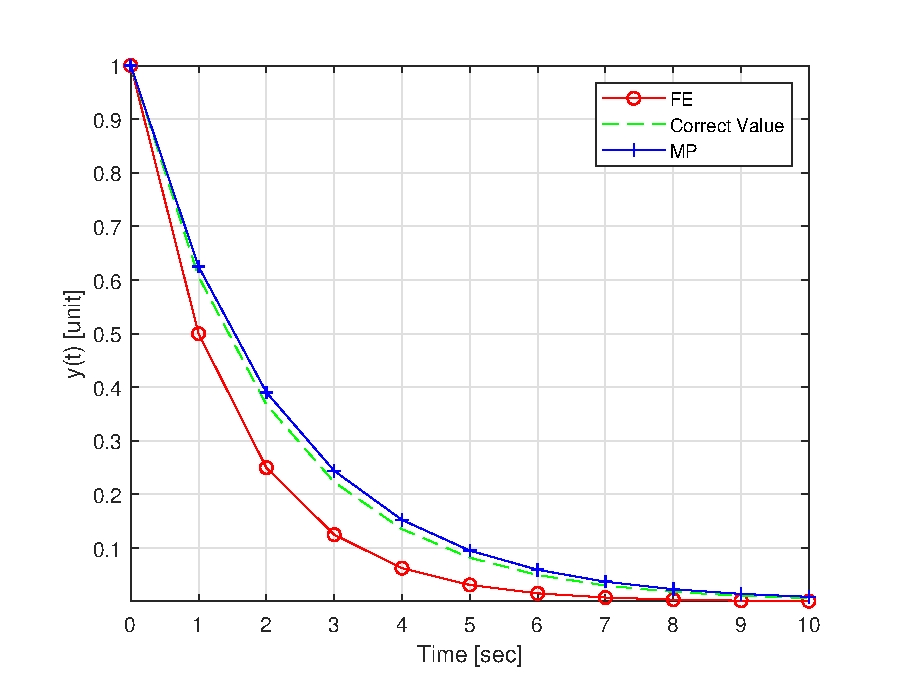
\includegraphics[width=0.7\textwidth]{graphics/six_mp.eps}
				\caption{Comperation between Forward Euler and Mid-Point-Method}
				\label{fig:sixmp}
			\end{figure}

	
		\subsection{Different h-Values}
		As in Section \ref{sec:val}, various values were also tested here. Up to the value h = 4, the MP method is more accurate. If h $\geq$ 5, the values of the MP method go in the wrong direction. However, the values do not oscillate with the MP method. This can be seen in Figure \ref{fig:sixc}.
		The reason for this is that $k1 * h / 2 = -1.25$. Thus, the point between t0 and t0 + h is regarded as being in the negative range.
		
		
			\begin{eqnarray}
				k1 = f\left( 0, 1, 2\right)  &= -0.5 \\
				k2 = f\left( 0, \frac{h}{2}, 1 + 5 * 2 \right) &= 0.125 \\
				yk_mp1 = 1 + 5 * 0.125 &= 1.625
			\end{eqnarray}
		
			\begin{figure} [H]
				\begin{center}
					\begin{subfigure}{0.3\textwidth}
						\begin{center}
							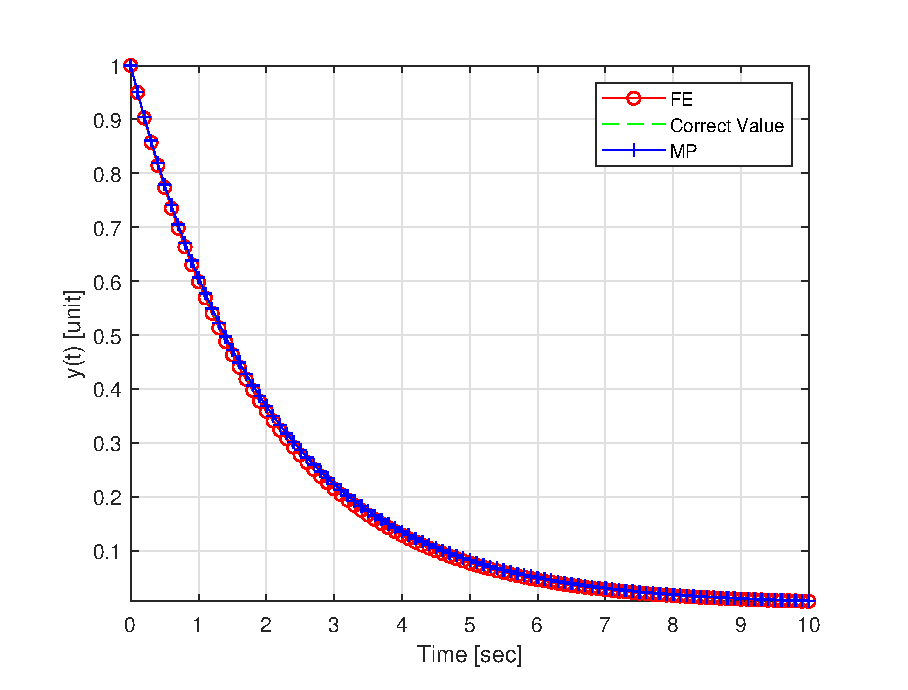
\includegraphics[width=1\textwidth]{graphics/sixc0_1.eps}
						\end{center}
					\end{subfigure}
					\begin{subfigure}{0.3\textwidth}
						\begin{center}
							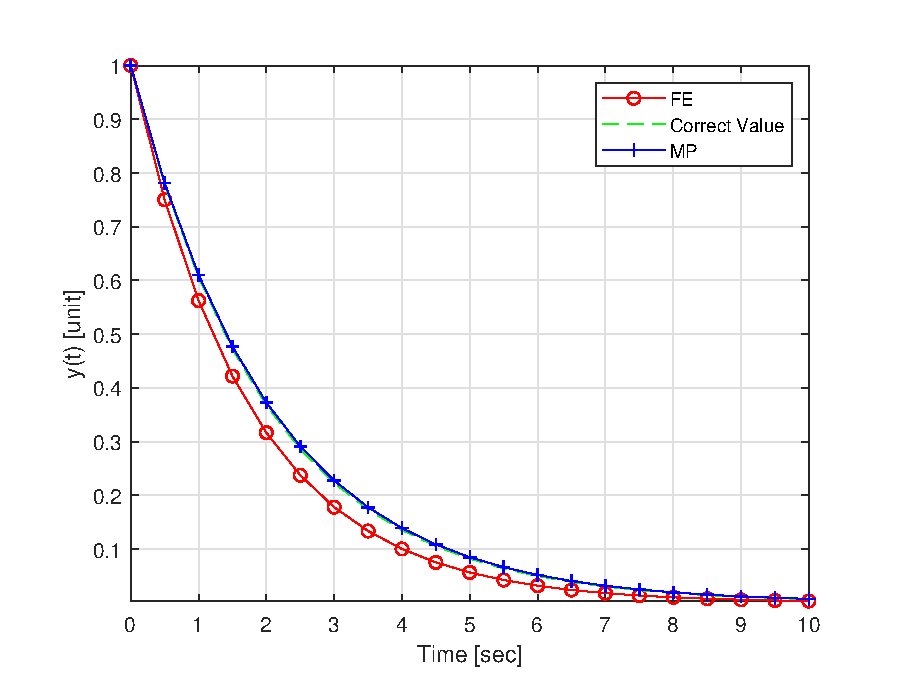
\includegraphics[width=1\textwidth]{graphics/sixc0_5.eps}
						\end{center}
					\end{subfigure}
					\begin{subfigure}{0.3\textwidth}
						\begin{center}
							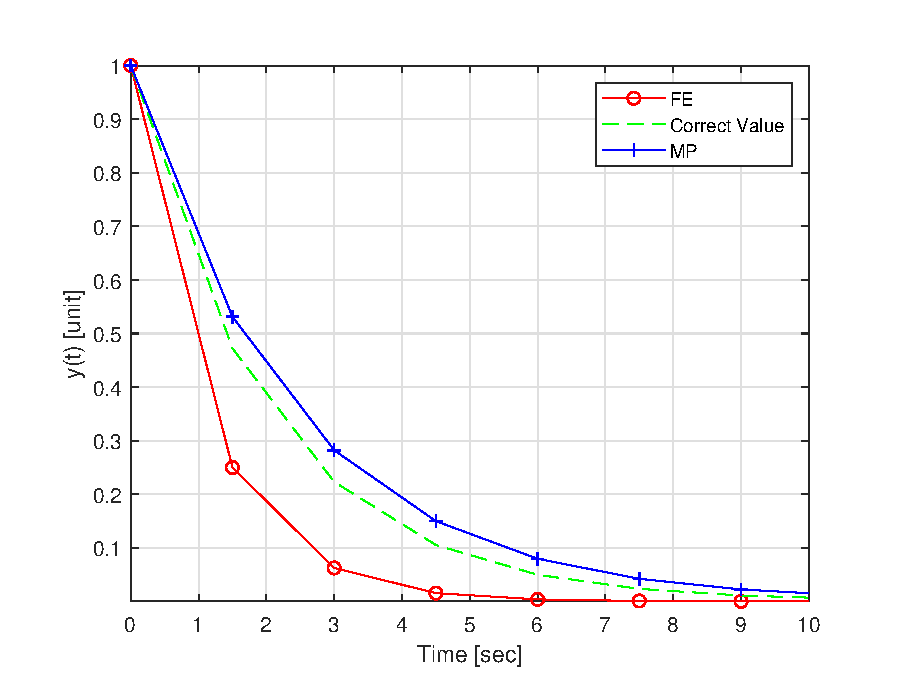
\includegraphics[width=1\textwidth]{graphics/sixc1_5.eps}
						\end{center}
					\end{subfigure}
					\begin{subfigure}{0.3\textwidth}
						\begin{center}
							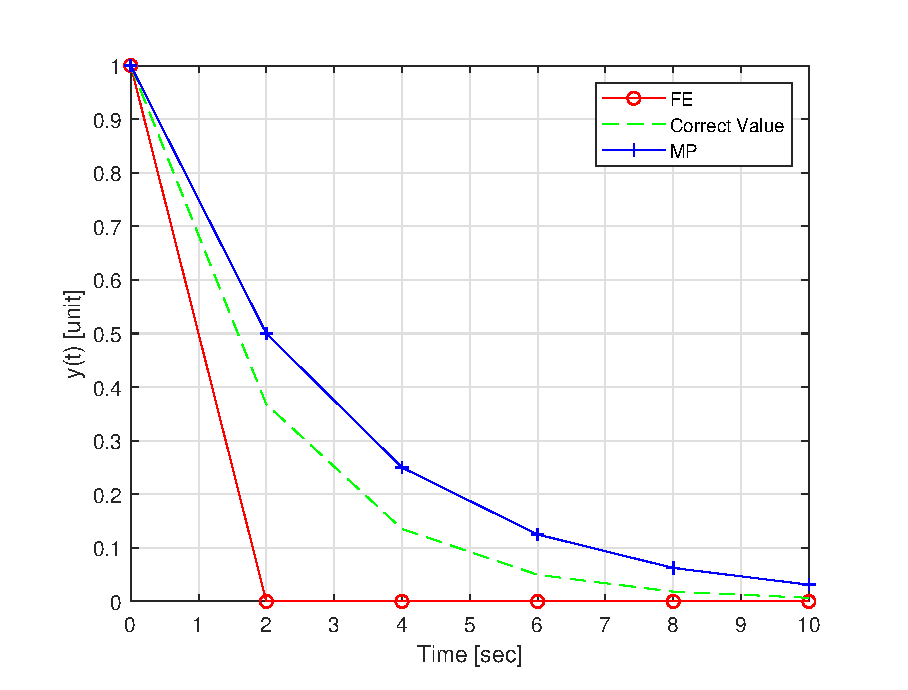
\includegraphics[width=1\textwidth]{graphics/sixc2.eps}
						\end{center}
					\end{subfigure}
					\begin{subfigure}{0.3\textwidth}
						\begin{center}
							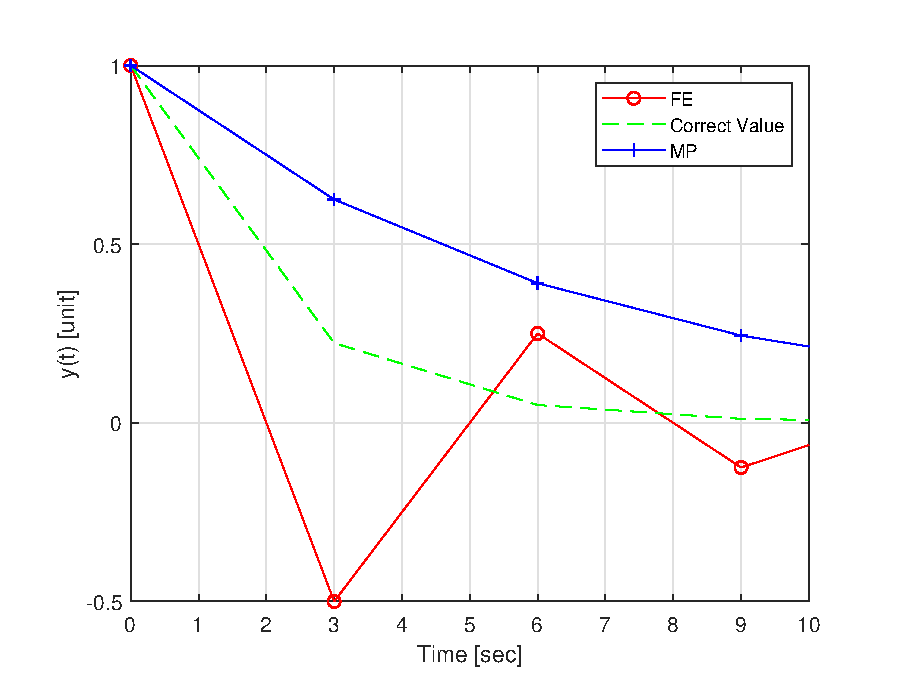
\includegraphics[width=1\textwidth]{graphics/sixc3.eps}
						\end{center}
					\end{subfigure}
					\begin{subfigure}{0.3\textwidth}
						\begin{center}
							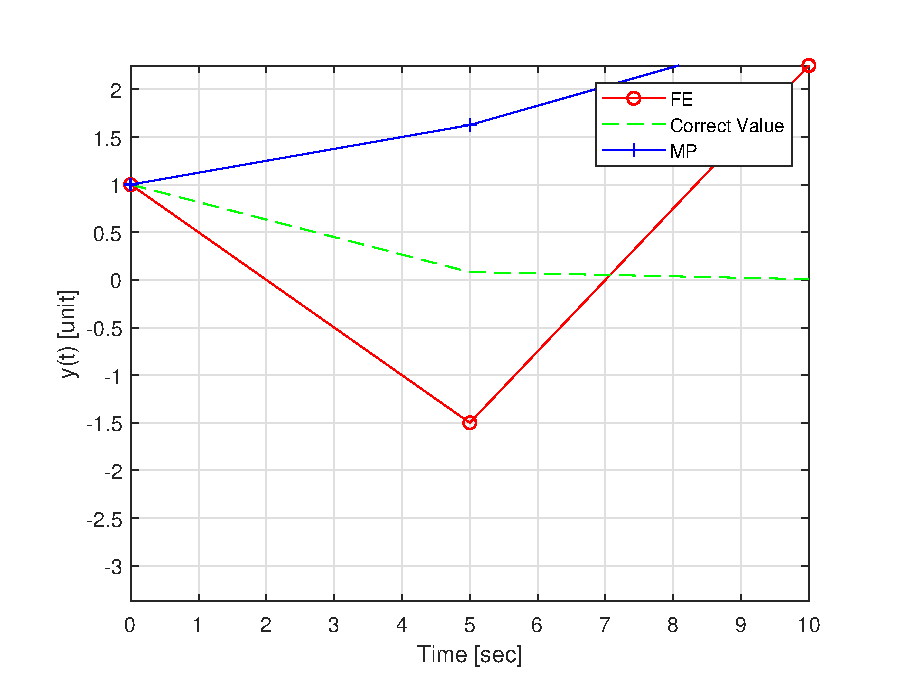
\includegraphics[width=1\textwidth]{graphics/sixc5.eps}
						\end{center}
					\end{subfigure}
					\caption[Different h-values]{Different h-values. From top left: 0.1, 0.5, 1.5, 2, 3, 5\\
						Quelle: Eigene Darstellung}
					\label{fig:sixc}
				\end{center}
			\end{figure}
	
	
	\section{Stepsize calculation}
	The tolerance parameter rtol was set to 0.1 and the relative error $\epsilon$ was calculated with Equation \ref{eq:3}. As soon as $\epsilon$ is smaller than rtol, the h-value is recalculated with Equation \ref{eq:4}.
	
		\begin{eqnarray}
			\epsilon  &=& \left| y_{k_{MP}} - y_{k_{FE}} \right| \label{eq:3}\\
			h &=& h * \sqrt{\frac{rtol}{\epsilon}} \label{eq:4}
		\end{eqnarray}
		

	
	\section{plot}
	The Figure \ref{fig:femp} was created with a rtol of 0.1. The code is in the appendix under Listing \ref{lst:ode12}. The innermost loop ran 213 times.
	
		\begin{figure}[H]
			\centering
			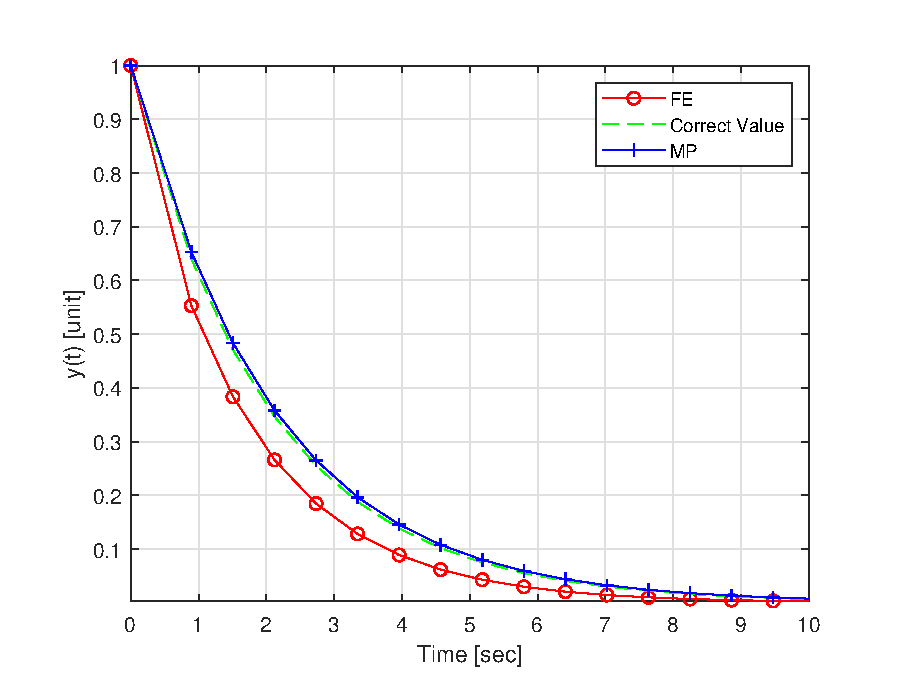
\includegraphics[width=0.7\textwidth]{graphics/seven_mp.eps}
			\caption{Variable h with an rtol of 0.1}
			\label{fig:femp}
		\end{figure}
	
	\section{Test of the solver with variable relative tolerance}
	If you double the accuracy, that is halving rtol, the number of loops and data points will be doubled.	This can be seen well in Figure \ref{fig:var_rtol} and Table \ref{tb:rtol}.
		
		\begin{table}[H]
			\begin{center}
			\begin{tabular}{c|ccccc}
				
				rtol 	& 0.2 & 0.1 & 0.05 & 0.025 & 0.0125\\ \hline
				loops	& 11 & 213 & 498 & 1059 & 2093 \\
				points  & 12 & 17 & 37 & 79 & 168 
				
			\end{tabular}
			\caption{Calculation effort with different rtol.}
			\label{tb:rtol}
			\end{center}
		\end{table}
	
		\begin{figure}[H]
			\centering
			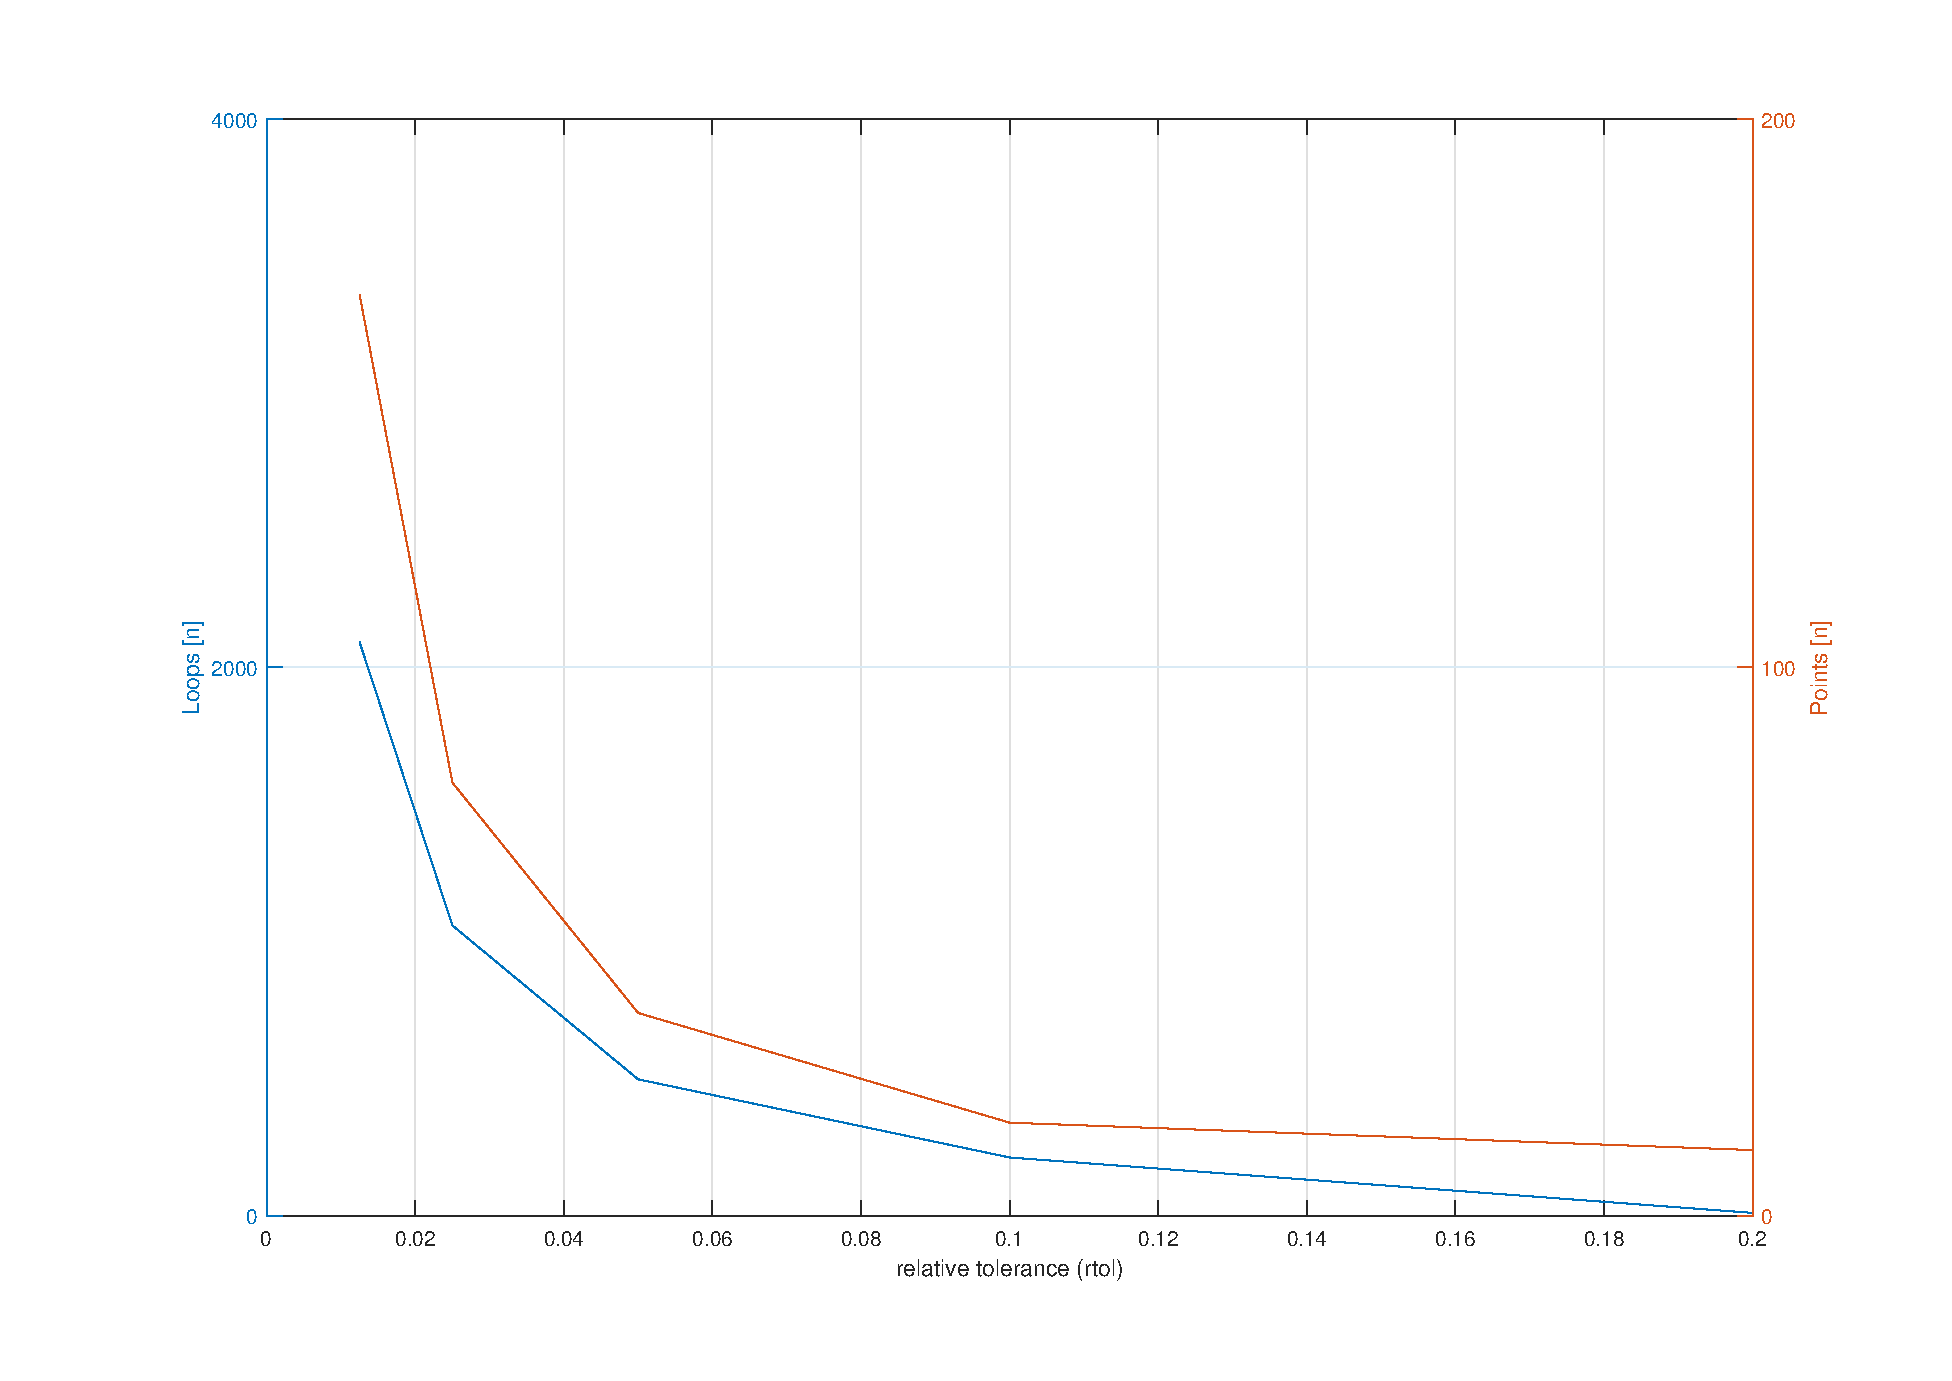
\includegraphics[width=0.7\textwidth]{graphics/var_rtos.eps}
			\caption{Points and loops depending on the relative tolerance.}
			\label{fig:var_rtol}
		\end{figure}

	%\section{Additional}

\part{Conclusion}
The simplest method is the Forward Euler or the Backwards Euler where the slope is recalculated at each point. However, this requires a lot of computing power when high accuracy is needed.
A bit more accurate is the mid-point method. In this a second algorithm is used to get a more accurate result.
Both methods have the disadvantage that they don 't adjust their step size if there are too large deviations. This was improved in task seven.


\newpage

\begin{appendices}

\begin{lstlisting}[caption={$test\_ode1$}, language=matlab, backgroundcolor = \color{lgray}, label={lst:ode1}]
	%%
	% This script implement Forward Euler method for solving a 
	%      ordinary differential equation defined by the function f
	%
	% Author: R.Estrada, FH JOANNEUM
	% Date:   May 2014
	%%
	
	
	%% Cleaning-up
	clear all; % Clean of variable-size matrices. Important to avoid "ghost" values
	cla;          % Clean active figure  
	
	%% Param definition
	y0 = 1;       % Initial condition of y
	t0 = 0;       % Initial time  
	tfinal = 10;  % Final time
	
	h = 5;        % Step size
	
	%% Main code
	% Variable init
	t = t0;                 % Actual time 
	i = 1;                  % Index counter 
	yk1(i,:) = [t0 y0 h];   % Matrix of result (first row)
	yk2(i,:) = [t0 y0 h];   %Matrix of 4a
	Tau = 2;                %4a Schaue Verhältniss h & Tau
	y_start =1;             %4a 
	abs_dif(i) = 0;
	dif(i) = 0;             %4c
	
	
	while 1                 % Infinite main loop
	
	% Forward Euler method (1st order)
	y1 = y0 + h*f(t,y0, Tau);
	
	% Updating values for next iteration
	y0 = y1;            
	i = i + 1;
	t = t + h;
	
	% Storing actual results
	yk1(i,:) = [t y1 h];
	
	%4a
	y_t = y_start*exp(-t/Tau);
	yk2(i,:) = [t y_t h]; 
	
	%4c
	abs_dif(i)  = abs(yk1(i,2)-yk2(i,2));
	dif(i)      = yk1(i,2)-yk2(i,2);
	
	
	
	% Ending condition
	if t > tfinal
	break;
	end    
	end
	
	%aav = sum(abs_dif)/(i-1);
	
	%Display of results
	figure(1)
	plot(yk1(:,1),yk1(:,2),'r');
	hold on
	plot(yk2(:,1),yk2(:,2), 'x');
	axis([t0 tfinal min(yk1(:,2)) max(yk1(:,2))]);
	xlabel('Time [sec]')
	ylabel('y(t) [unit]')
	legend('FE', 'EstVal');
	grid
	hold off
	
	arr4 = [yk1(:,1), yk1(:,2), yk2(:,2), (yk2(:,2)-yk1(:,2))];
	aate4 = sum(abs(arr4(:,4)))/(length(arr4)-1);
	rms4 = rms(arr4(2:end,4))
	% latex(vpa(sym(array_latex),3));
	
	
	
	errors = [0.1, 0.5, 1.5, 2, 3, 5; 0.0048, 0.0243, 0.0796, 0.0968, 0.2799, 2.4003;...
	0.0056, 0.0296, 0.1109, 0.1615, 0.3825, 2.5119];
	
	figure(2)
	plot(errors(1,:),errors(2,:),'o-');
	hold on
	plot(errors(1,:),errors(3,:), 'x-');
	axis([0 5 0 2.6]);
	xlabel('h [sec]')
	ylabel('Error []')
	legend('AATE', 'RMS');
	grid
	hold off
\end{lstlisting}

\newpage
\begin{lstlisting}[caption={$test\_ode1$}, language=matlab, backgroundcolor = \color{lgray}, label={lst:ode12}]
	%%
	% This script implement Forward Euler method for solving a 
	%      ordinary differential equation defined by the function f
	%
	% Author: R.Estrada, FH JOANNEUM
	% Date:   May 2014
	%%
	
	
	%% Cleaning-up
	clear all; % Clean of variable-size matrices. Important to avoid "ghost" values
	cla;          % Clean active figure  
	
	%% Param definition
	%FE
	y0 = 1;       % Initial condition of y
	
	%MP
	yk_mp = 1;      %initial Value
	yk_mp1 = 1;     %yk_mp+1
	
	%General
	t0 = 0;       % Initial time  
	tfinal = 10;  % Final time
	
	h = 1;        % Step size
	rtol = 0.1;     %6
	
	%% Main code
	% Variable init
	t = t0;                 % Actual time 
	i = 1;                  % Index counter 
	yk1(i,:) = [t0 y0 h];   % Matrix of result (first row)
	yk2(i,:) = [t0 y0 h];   %Matrix of 4a
	yk3(i,:) = [t0 y0 h];   %6
	Tau = 2;                %4a Schaue Verhältniss h & Tau
	y_start =1;             %4a 
	abs_dif1(i) = 0;        %4a
	dif(i) = 0;             %4c
	j=0;                    % n loops
	h_i(i) = [1];           % stepsize
	
	
	
	while 1                 % Infinite main loop
	
	k1 = 0;                 %7
	k2 = 0;                 %7
	
	while 1
	j = j+1;
	% Forward Euler method (1st order)
	y1 = y0 + h*f(t,y0, Tau);
	
	
	
	%MP Mid-Point Method 
	%6
	k1  = f(t,yk_mp, Tau);
	k2  = f(t + h/2, yk_mp + k1*h/2, Tau);  
	yk_mp1 = yk_mp + h * k2;
	
	%solve epsilon
	epsilon = abs(yk_mp1 - y1);
	
	if epsilon <= rtol
	break;
	else 
	h = h * sqrt(rtol/epsilon);
	end      
	end
	
	
	% Updating values for next iteration
	%yk1
	y0 = y1;            
	%yk2
	%yk3      
	yk_mp = yk_mp1;%yk_mp + h * k2;
	%general
	i = i + 1;
	t = t + h;
	
	% Storing actual results
	yk1(i,:) = [t y1 h];
	yk3(i,:) = [t yk_mp1 h];
	h_i(i) = h;
	
	% Correct Value
	%4a
	y_t = y_start*exp(-t/Tau);
	yk2(i,:) = [t y_t h]; 
	
	
	
	%4c
	abs_dif1(i)  = abs(yk1(i,2)-yk2(i,2));
	dif1(i)      = yk1(i,2)-yk2(i,2);
	
	
	
	%         abs_dif2(i)  = abs(yk3(i,2)-yk2(i,2));
	%         dif1(2)      = yk3(i,2)-yk2(i,2);
	
	
	% Ending condition
	if t > tfinal
	break;
	end 
	
	end
	
	% aav = sum(abs_dif1)/(i-1);
	% 
	% 
	% 
	% aav2 = sum(abs_dif2)/(i-1);
	
	% Display of results
	plot(yk1(:,1),yk1(:,2),'ro-');
	hold on
	plot(yk2(:,1),yk2(:,2), 'g--');
	plot(yk3(:,1),yk3(:,2), 'b+-');
	axis([t0 tfinal min(yk1(:,2)) max(yk1(:,2))]);
	xlabel('Time [sec]')
	ylabel('y(t) [unit]')
	legend('FE', 'Correct Value', 'MP');
	grid
	hold off
\end{lstlisting}	
		
\end{appendices}